% Asset ID: FA22SimplexAlgorithmTableauTikZ-001
% Unit: FA22 Further A2 2 Applied Mathematics
% Applied section: Section D, Discrete and Decision Mathematics
% Topic code: FA22-ALGGRAPH
% Topic ID: FA22SimplexAlgorithmTableau
% Related LO: FA22-ALGGRAPH-LO003
% Related lesson file: FA22_simplex_algorithm_tableau_lesson.md
% Related lesson section: #9. Visual Asset Integration
% Used placeholder:
% [VISUAL PLACEHOLDER: FA22SimplexAlgorithmTableauTikZ-001 | Source: Two-variable simplex example evidence | Insert from tikz/FA22SimplexAlgorithmTableauTikZ-001.tex | Purpose: Provide a mathematically precise graph for the worked example.]
% Source: Two-variable simplex example evidence
% Purpose: Provide a mathematically precise graph for the worked example.
% Creation status: Generated in Phase 4
% On-spec status: Core CCEA Further Mathematics content, restricted to two-variable linear programming problems.

\documentclass[tikz,border=8pt]{standalone}
\usepackage{amsmath,amssymb}
\usetikzlibrary{arrows.meta,calc,positioning}
\definecolor{Canvas}{HTML}{FAF9F6}
\definecolor{Panel}{HTML}{FFFFF0}
\definecolor{LineSoft}{HTML}{E5E5EA}
\definecolor{Accent}{HTML}{C5A059}
\definecolor{AccentDeep}{HTML}{D4AF37}
\definecolor{TextDark}{HTML}{2C2C2E}
\definecolor{SoftRose}{HTML}{FBEFEF}
\definecolor{ConstraintA}{HTML}{8E8E93}
\definecolor{ConstraintB}{HTML}{6E6E73}
\begin{document}
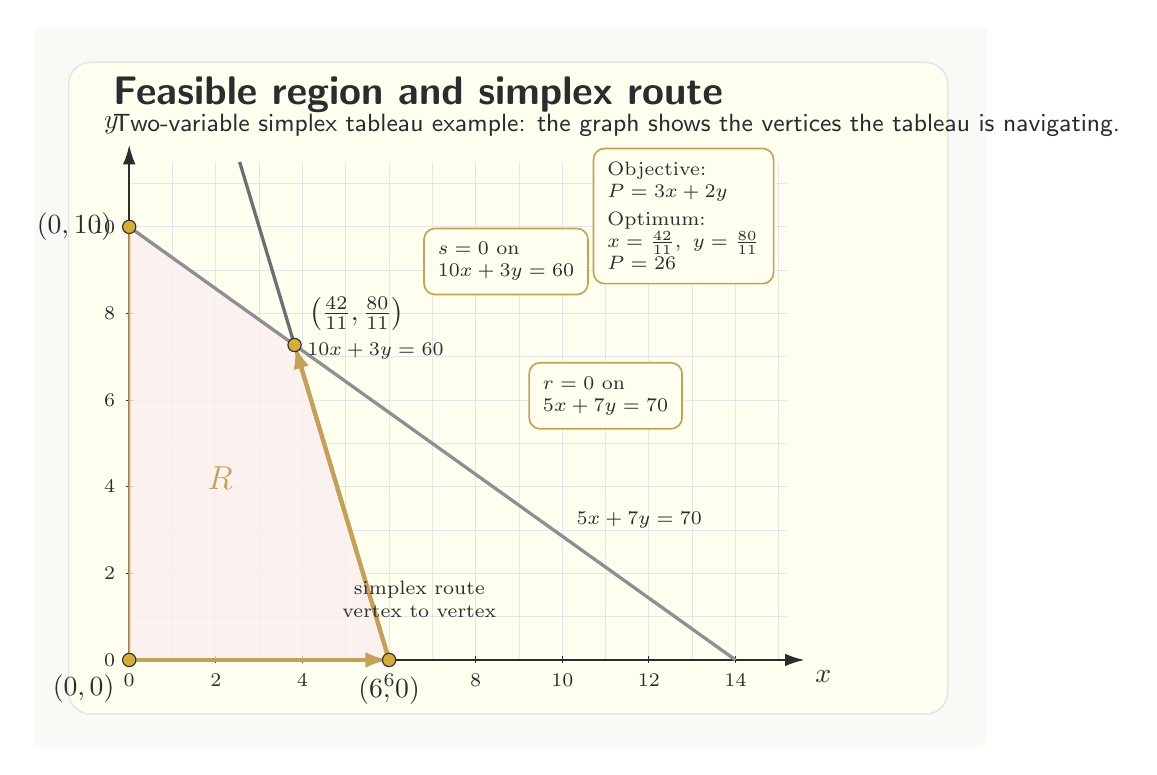
\begin{tikzpicture}[x=0.55cm,y=0.55cm,every node/.style={font=\sffamily,text=TextDark},axis/.style={draw=TextDark,line width=0.9pt},gridline/.style={draw=LineSoft,line width=0.35pt},route/.style={draw=Accent,line width=1.6pt,-{Latex[length=3mm,width=2mm]}},vertex/.style={circle,draw=TextDark,fill=AccentDeep,inner sep=1.7pt},note/.style={draw=Accent,fill=Panel,rounded corners=4pt,line width=0.6pt,align=left,inner sep=5pt}]
\fill[Canvas] (-2.2,-2.0) rectangle (19.8,14.6);
\filldraw[fill=Panel,draw=LineSoft,line width=0.6pt,rounded corners=8pt] (-1.4,-1.25) rectangle (18.9,13.8);
\node[anchor=west,font=\sffamily\bfseries\Large] at (-0.6,13.05) {Feasible region and simplex route};
\node[anchor=west,font=\sffamily\small] at (-0.6,12.35) {Two-variable simplex tableau example: the graph shows the vertices the tableau is navigating.};
\foreach \x in {0,1,...,15}{\draw[gridline](\x,0)--(\x,11.5);} \foreach \y in {0,1,...,11}{\draw[gridline](0,\y)--(15.2,\y);}
\draw[axis,-{Latex[length=2.5mm,width=1.6mm]}](0,0)--(15.6,0) node[below right]{$x$};
\draw[axis,-{Latex[length=2.5mm,width=1.6mm]}](0,0)--(0,11.9) node[above left]{$y$};
\foreach \x in {0,2,4,6,8,10,12,14}{\draw[TextDark](\x,0.08)--(\x,-0.08);\node[below,font=\scriptsize] at (\x,-0.10){$\x$};}
\foreach \y in {0,2,4,6,8,10}{\draw[TextDark](0.08,\y)--(-0.08,\y);\node[left,font=\scriptsize] at (-0.10,\y){$\y$};}
\coordinate (O) at (0,0); \coordinate (A) at (6,0); \coordinate (B) at ({42/11},{80/11}); \coordinate (C) at (0,10); \coordinate (D) at (14,0); \coordinate (E) at (2.55,11.5);
\filldraw[fill=SoftRose,opacity=0.76,draw=Accent,line width=0.8pt] (O)--(A)--(B)--(C)--cycle;
\draw[draw=ConstraintA,line width=1.2pt] (C)--(D) node[pos=0.72,above right,font=\scriptsize]{$5x+7y=70$};
\draw[draw=ConstraintB,line width=1.2pt] (E)--(A) node[pos=0.38,right,font=\scriptsize]{$10x+3y=60$};
\draw[route] (O)--(A); \draw[route] (A)--(B);
\node[vertex,label=below left:{$(0,0)$}] at (O){}; \node[vertex,label=below:{$(6,0)$}] at (A){}; \node[vertex,label=above right:{$\left(\frac{42}{11},\frac{80}{11}\right)$}] at (B){}; \node[vertex,label=left:{$(0,10)$}] at (C){};
\node[note,font=\scriptsize] at (11.0,6.1){$r=0$ on\\$5x+7y=70$};
\node[note,font=\scriptsize] at (8.7,9.2){$s=0$ on\\$10x+3y=60$};
\node[note,font=\scriptsize] at (12.8,10.25){Objective:\\$P=3x+2y$\\[2pt]Optimum:\\$x=\frac{42}{11},\ y=\frac{80}{11}$\\$P=26$};
\node[font=\sffamily\bfseries\large,text=Accent] at (2.1,4.2){$R$};
\node[font=\scriptsize,align=center] at (6.7,1.4){simplex route\\vertex to vertex};
\end{tikzpicture}
\end{document}
